\section[约束秩亏问题]{约束秩亏问题\\Constraining a rank Deficient Problem}	
When $A$ has dependent columns, there are an infinite number of solutions (differing by the solutions of $Ax= \mathbf{0}$) to the singular least-squares problem:
\begin{center}
	Choose $\hat{x}$ to minimize $||{x - Ax}||$.
\end{center}
We look for a unique solution $\hat{x}$ by imposing \emph{d} additional constraints
\begin{equation}
	G^\mathsf{T}x
	=g
\end{equation}
Here $d = n - r$ = number of columns in $A$ minus number of independent columns(the rank).Then $A$ augmented by the $d$ new columns from  $G$ has full rank $n$.
\par
We formulate the problem as one consisting of a singular matrix $A^\mathsf{T}A$ with \emph{an orthogonal bordering} matrix $G$:
\begin{equation}
	\begin{bmatrix}
		A^\mathsf{T}A & G \\
		G^\mathsf{T} & \mathbf{0}
	\end{bmatrix}
	\begin{bmatrix}
		x\\
		\mathbf{0}
	\end{bmatrix}
	=
	\begin{bmatrix}
		A^\mathsf{T}b \\ g
	\end{bmatrix}.
\end{equation}
\par\noindent
The augmentation of $A^\mathsf{T}A$ by $G^\mathsf{T}$ makes the block matrix invertible.The solution is unique,and it can be expressed in terms of the pseudoinverse  $A^\mathsf{+}$:
\begin{equation}
	x^\mathsf{+}
	=A^\mathsf{+}b.
\end{equation}
\textbf{Remark 7.2} There is another formulation of the problem. Let the normal equations be
\begin{equation}
	A^\mathsf{T}Ax
	=A^\mathsf{T}b.
\end{equation}
$A^\mathsf{T}A$ is still singular and nonnegative definite. In order to make the problem uniquely solvable we add a suitable set of $d$ fictitious \emph{observation equations}
\begin{equation}
	Fx
	=g.
\end{equation}
Now we consider the unweighted least-squares problem for the matrix
$\begin{bmatrix}
A\\
F
\end{bmatrix}$
with full column rank. Suppose these observation equations are weight normalized such that the normals become
\begin{equation}
	(A^\mathsf{T}A + F^\mathsf{T}F)x
	=A^\mathsf{T}b + F^\mathsf{T}g.
\end{equation}
Such an addition to the problem is called a \emph{soft postulation}. We shall see how the inverse of the coefficient matrix depends on this soft postulation.
\par
If the fictitious observations are given infinite weight��\emph{hard postulation}, which implies that (7.18) is strictly enforced��then those are regarded as \emph{condition equations} and not as observation equations.
\par
We demonstrate the technique on the transformation (7.44) below and modify it for a soft postulation as follows
\begin{equation}
	\sum\nolimits_{\text{transformed}}
	=S(\sum\nolimits_{\hat{x}} + G^\mathsf{T})S^\mathsf{T}.
\end{equation}
according to Krarup (1979).
\par\noindent
\textbf{Example 7.2} Let the oriented graph in Figure 7.2 and height differences along the edges be given. The incidence matrix corresponding to this graph is
\begin{equation*}
	A
	=
	\begin{bmatrix}
		-1 & 0 & 0 & 1 & 0\\
		-1 & 0 & 0 & 0 & 1\\
		0 & 0 &-1 & 1 & 0\\
		0 &-1 & 0 & 0 & 1\\
		0 & 0 & 0 & 1 & -1
	\end{bmatrix}
\end{equation*}
with the observations
\begin{equation*}
	b
	=
	\begin{bmatrix}
		1.978\\
		0.732\\
		0.988\\
		0.420\\
		1.258
	\end{bmatrix}.
\end{equation*}
\begin{figure}
	\centering
	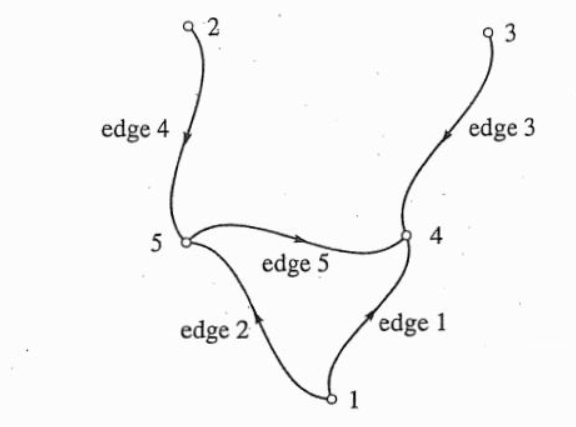
\includegraphics[width=0.4\linewidth]{TeX_files/Part02/chapter07/image/7-2.png}
	\caption{Figure 7.2 Graph for oriented free leveling network}
	\label{fig:7-2}
\end{figure}
The matrix $A^\mathsf{T}A$ is singular.$A$ unique solution can be calculated by means of the pseudoinverse matrix $A^\mathsf{+}$. This matrix is often determined by means of the SVD for $A$. This is the decomposition $A = U\sum V^\mathsf{T}$ and the pseudoinverse is explained in Section 7.1: $A^+ = V\sum^{+}U^\mathsf{T}$. The unique least-squares solution of minimum norm is
\begin{equation*}
	x^+
	= A^{+}b
	=
	\begin{bmatrix}
		-0.8024\\
		-0.4944\\
		0.1916\\
		1.1796\\
		-0.0744
	\end{bmatrix}.
\end{equation*}
The same solution $\hat{x} = x^{+}$ can be achieved by augmenting $A^\mathsf{T}A$ by the row $e^\mathsf{T}$ and the
column $e$ of all ones, taken from the nullspace of $A$:
\begin{equation*}
	\begin{bmatrix}
		A^\mathsf{T}A & e \\
		e^\mathsf{T} & \mathbf{0}
	\end{bmatrix}
	\begin{bmatrix}
		x\\
		\mathbf{0}
	\end{bmatrix}
	=
	\begin{bmatrix}
		A^\mathsf{T}b \\
		\mathbf{0}
	\end{bmatrix}.
\end{equation*}
Note that the mean value of $\hat{x} = \hat{x}_{0}$ is zero. This gives the last equation $e^\mathsf{T}\hat{x} = \mathbf{0}$. To find the solution we did not form the normal equations but rather used the SVD.
\par
If we want to change the solution $\hat{x}_{0}$ from "0-level" to a level such as $l$ = 20, we simply have to change $g$ to 5 $\times$ 20 = 100 and we obtain the solution
\begin{equation*}
	\hat{x}_{20}
	=     \begin{bmatrix}
		19.1976\\
		19.5056\\
		20.1916\\
		21.1796\\
		19.9256
	\end{bmatrix}.
\end{equation*}
The mean value of this solution is 20 because $e^\mathsf{T}\hat{x}_{20} = 100$.
\par\noindent
\textbf{Example 7.3} We want to demonstrate how a projector can bring $\hat{x}_{20}$ from Example 7.2 back to $\hat{x}_{0}$. In this special case we project onto the plane perpendicular to $e$. The projection matrix is
\begin{equation*}
	P
	= I - e(e^\mathsf{T}e)^{-1}e^\mathsf{T}
	= I - \frac{1}{5}ee^\mathsf{T}
	= \frac{1}{5}
	\begin{bmatrix}
		4 & -1 & -1 & -1 & -1\\
		-1 & 4  & -1 & -1 & -1\\
		-1 & -1 &  4 & -1 & -1\\
		-1 & -1 & -1 &  4 & -1\\
		-1 & -1 & -1 & -1 & 4\\
	\end{bmatrix}
\end{equation*}
or
\begin{equation*}
	\hat{x}_{0}
	=P\hat{x}_{20}
	= p
	\begin{bmatrix}
		19.1976\\
		19.5056\\
		20.1916\\
		21.1796\\
		19.9256
	\end{bmatrix}
	=\begin{bmatrix}
		-0.8024\\
		-0.4944\\
		0.1916\\
		1.1796\\
		-0.0744
	\end{bmatrix}.
\end{equation*}
\textbf{Example 7.4} Continuing Example 7.2 we shall calculate the covariance matrix for the
pseudoinverse solution. We shall determine the standard deviation (of unit weight)
$b - Ax^{+} = b - AA^{+}b
= (I - AA^{+})b$
and $\hat{\sigma}_0 = ||b - Ax^{+}||
= 0.0069 = 6.9mm.$
\par\noindent
Thus the covariance matrix $\Sigma_+ = {\hat{\sigma}_0}^2\emph{A}^{+}(\emph{A}^{+})^\mathsf{T}$ is
\begin{equation*}
	\begin{bmatrix}
		0.192 & -0.096 & -0.096 & -0.000 & -0.000\\
		-0.096 & 0.416  & -0.224 & -0.128 & 0.032\\
		-0.096 & -0.224 & 0.416  & 0.032  & -0.128\\
		-0.000 & -0.128 & 0.032  & 0.128  & -0.032\\
		-0.000 & 0.032  & -0.128 & -0.032 & 0.128\\
	\end{bmatrix}\times10^{-4}.
\end{equation*}
with trace$(\sum_+) = 1.280 \times 10^{-4}$. Next we have
\begin{equation*}
	Bx
	=
	\begin{bmatrix}
		A\\
		e^\mathsf{T}
	\end{bmatrix}
	x
	=
	\begin{bmatrix}
		b\\
		\mathbf{0}
	\end{bmatrix}
\end{equation*}
and $\sum = {\hat{\sigma}_0}^2(B^\mathsf{T}B)^{-1}$ becomes
\begin{equation*}
	\begin{bmatrix}
		0.211 &-0.077 &-0.077 &0.019  &0.019\\
		-0.077 &0.435  &-0.205 &-0.109 &0.051\\
		-0.077 &-0.205 &0.435  &0.051  &-0.109\\
		0.019 &-0.109 &0.051  &0.147  &-0.013\\
		0.019  &0.051  &-0.109 &-0.013 &0.147\\
	\end{bmatrix}\times10^{-4}.
\end{equation*}
Finally trace$(\sum) = 1.376 \times 10^{-4}$. Obviously trace$(\sum_+)$$ <$ trace$(\sum)$.
\par\noindent
\textbf{Example 7.5} This is the example of a \emph{free network}. We augment the original $n = 2$ unknowns to include the unknowns of all other points in the network. Hence the number of unknowns increases to 8. As rank$(A) = 8 - 3 = 5$ we have to include at least two.
\begin{figure}
	\centering
	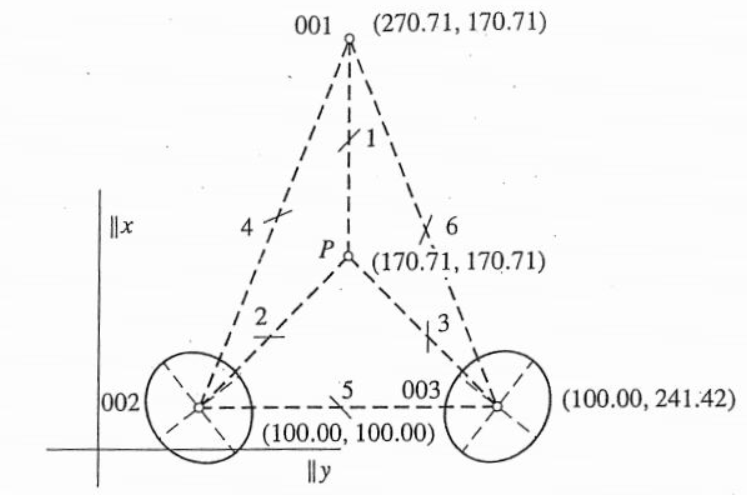
\includegraphics[width=0.4\linewidth]{TeX_files/Part02/chapter07/image/7-3.png}
	\caption{}
	\label{fig:7-3}
\end{figure}
\par\noindent
\textbf{Figure 7.3} Free distance network with 6 observations. The confidence ellipses correspond to the postulated coordinates $X_P$,$Y_P$,$X_{001}$,and $Y_{001}$.
\par\noindent
more observations compared to Example 7.1. For reasons of symmetry we include even three more observations, viz. distance observations between the pairs 001-002, 002-003,and 003-001. The vector of unknowns is
\begin{equation*}
	x =
	\begin{pmatrix}
		x_P,y_P,x_{001},y_{001},x_{002},
		y_{002},x_{003},y_{003}
	\end{pmatrix}.
\end{equation*}
The augmented coefficient matrix is 6 by 8 with rank 4:
\begin{equation*}
	A =
	\begin{bmatrix}
		-1 & 0 & 1 & 0 & 0 & 0 & 0 & 0\\
		0.707 & 0.707 & 0 & 0 & -0.707 & -0.707 & 0 & 0\\
		0.707 &-0.707& 0 &0 &0& 0& -0.707& 0.707\\
		0 & 0 &0.924& 0.383& -0.924 &-0.383& 0& 0\\
		0& 0 &0 &0 &0 &-1& 0& 1\\
		0& 0 &0.924 &-0.383& 0& 0&\ -0.924& 0.383
	\end{bmatrix}.
\end{equation*}
We choose a basis for the nullspace of dimension 4, in the rows of $G^\mathsf{T}$:
\begin{equation*}
	G^\mathsf{T} =
	\begin{bmatrix}
		1 & 0 & 1 & 0 & 1 & 0 & 1 & 0\\
		0 & 1 & 0 & 1 & 0 & 1 & 0 & 1\\
		-170.71 & 170.71 &-170.71& 270.71& -100 &100& -241.42& 100\\
		\quad170.71& 170.71 &\quad270.71 &170.71& \quad100& 100& 100& \quad241.42
	\end{bmatrix}.
\end{equation*}
and the right side is
\begin{equation*}
	b
	=\begin{bmatrix}
		0.010\\
		0.020\\
		0.030\\
		0.010\\
		0.020\\
		0.030
	\end{bmatrix}.
\end{equation*}
The pseudoinverse solution $x^+ = A^+b$ and the residuals $b - Ax^+$ are
\begin{equation*}
	b
	=\begin{bmatrix}
		\quad 0.008 0\\
		\quad0.002 3\\
		\quad0.0113\\
		-0.0068\\
		-0.0026\\
		-0.0087\\
		-0.0167\\
		0.013 2
	\end{bmatrix}
	\qquad \text{and}  \qquad
	b- Ax^+
\end{equation*}	
When $A$ has dependent columns, there are an infinite number of solutions (differing by the solutions of $Ax= \mathbf{0}$) to the singular least-squares problem:
\begin{center}
	Choose $\hat{x}$ to minimize $||{x - Ax}||$.
\end{center}
We look for a unique solution $\hat{x}$ by imposing \emph{d} additional constraints
\begin{equation}
	G^\mathsf{T}x
	=g
\end{equation}
Here $d = n - r$ = number of columns in $A$ minus number of independent columns(the rank).Then $A$ augmented by the $d$ new columns from  $G$ has full rank $n$.
\par
We formulate the problem as one consisting of a singular matrix $A^\mathsf{T}A$ with \emph{an orthogonal bordering} matrix $G$:
\begin{equation}
	\begin{bmatrix}
		A^\mathsf{T}A & G \\
		G^\mathsf{T} & \mathbf{0}
	\end{bmatrix}
	\begin{bmatrix}
		x\\
		\mathbf{0}
	\end{bmatrix}
	=
	\begin{bmatrix}
		A^\mathsf{T}b \\ g
	\end{bmatrix}.
\end{equation}
\par\noindent
The augmentation of $A^\mathsf{T}A$ by $G^\mathsf{T}$ makes the block matrix invertible.The solution is unique,and it can be expressed in terms of the pseudoinverse  $A^\mathsf{+}$:
\begin{equation}
	x^\mathsf{+}
	=A^\mathsf{+}b.
\end{equation}
\textbf{Remark 7.2} There is another formulation of the problem. Let the normal equations be
\begin{equation}
	A^\mathsf{T}Ax
	=A^\mathsf{T}b.
\end{equation}
$A^\mathsf{T}A$ is still singular and nonnegative definite. In order to make the problem uniquely solvable we add a suitable set of $d$ fictitious \emph{observation equations}
\begin{equation}
	Fx
	=g.
\end{equation}
Now we consider the unweighted least-squares problem for the matrix
$\begin{bmatrix}
A\\
F
\end{bmatrix}$
with full column rank. Suppose these observation equations are weight normalized such that the normals become
\begin{equation}
	(A^\mathsf{T}A + F^\mathsf{T}F)x
	=A^\mathsf{T}b + F^\mathsf{T}g.
\end{equation}
Such an addition to the problem is called a \emph{soft postulation}. We shall see how the inverse of the coefficient matrix depends on this soft postulation.
\par
If the fictitious observations are given infinite weight��\emph{hard postulation}, which implies that (7.18) is strictly enforced��then those are regarded as \emph{condition equations} and not as observation equations.
\par
We demonstrate the technique on the transformation (7.44) below and modify it for a soft postulation as follows
\begin{equation}
	\sum\nolimits_{\text{transformed}}
	=S(\sum\nolimits_{\hat{x}} + G^\mathsf{T})S^\mathsf{T}.
\end{equation}
according to Krarup (1979).
\par\noindent
\textbf{Example 7.2} Let the oriented graph in Figure 7.2 and height differences along the edges be given. The incidence matrix corresponding to this graph is
\begin{equation*}
	A
	=
	\begin{bmatrix}
		-1 & 0 & 0 & 1 & 0\\
		-1 & 0 & 0 & 0 & 1\\
		0 & 0 &-1 & 1 & 0\\
		0 &-1 & 0 & 0 & 1\\
		0 & 0 & 0 & 1 & -1
	\end{bmatrix}
\end{equation*}
with the observations
\begin{equation*}
	b
	=
	\begin{bmatrix}
		1.978\\
		0.732\\
		0.988\\
		0.420\\
		1.258
	\end{bmatrix}.
\end{equation*}
\begin{figure}
	\centering
	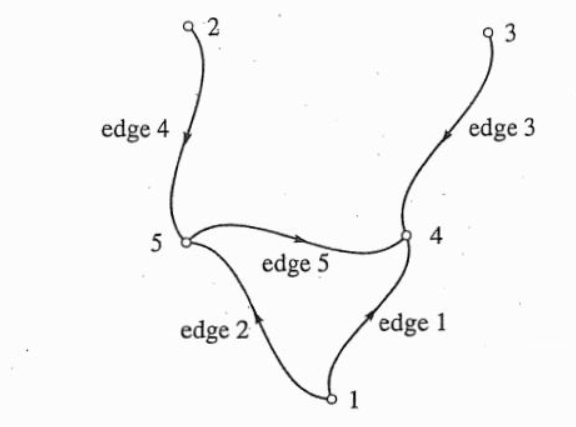
\includegraphics[width=0.4\linewidth]{TeX_files/Part02/chapter07/image/7-2.png}
	\caption{Figure 7.2 Graph for oriented free leveling network}
	\label{fig:7-2}
\end{figure}
The matrix $A^\mathsf{T}A$ is singular.$A$ unique solution can be calculated by means of the pseudoinverse matrix $A^\mathsf{+}$. This matrix is often determined by means of the SVD for $A$. This is the decomposition $A = U\sum V^\mathsf{T}$ and the pseudoinverse is explained in Section 7.1: $A^+ = V\sum^{+}U^\mathsf{T}$. The unique least-squares solution of minimum norm is
\begin{equation*}
	x^+
	= A^{+}b
	=
	\begin{bmatrix}
		-0.8024\\
		-0.4944\\
		0.1916\\
		1.1796\\
		-0.0744
	\end{bmatrix}.
\end{equation*}
The same solution $\hat{x} = x^{+}$ can be achieved by augmenting $A^\mathsf{T}A$ by the row $e^\mathsf{T}$ and the
column $e$ of all ones, taken from the nullspace of $A$:
\begin{equation*}
	\begin{bmatrix}
		A^\mathsf{T}A & e \\
		e^\mathsf{T} & \mathbf{0}
	\end{bmatrix}
	\begin{bmatrix}
		x\\
		\mathbf{0}
	\end{bmatrix}
	=
	\begin{bmatrix}
		A^\mathsf{T}b \\
		\mathbf{0}
	\end{bmatrix}.
\end{equation*}
Note that the mean value of $\hat{x} = \hat{x}_{0}$ is zero. This gives the last equation $e^\mathsf{T}\hat{x} = \mathbf{0}$. To find the solution we did not form the normal equations but rather used the SVD.
\par
If we want to change the solution $\hat{x}_{0}$ from "0-level" to a level such as $l$ = 20, we simply have to change $g$ to 5 $\times$ 20 = 100 and we obtain the solution
\begin{equation*}
	\hat{x}_{20}
	=     \begin{bmatrix}
		19.1976\\
		19.5056\\
		20.1916\\
		21.1796\\
		19.9256
	\end{bmatrix}.
\end{equation*}
The mean value of this solution is 20 because $e^\mathsf{T}\hat{x}_{20} = 100$.
\par\noindent
\textbf{Example 7.3} We want to demonstrate how a projector can bring $\hat{x}_{20}$ from Example 7.2 back to $\hat{x}_{0}$. In this special case we project onto the plane perpendicular to $e$. The projection matrix is
\begin{equation*}
	P
	= I - e(e^\mathsf{T}e)^{-1}e^\mathsf{T}
	= I - \frac{1}{5}ee^\mathsf{T}
	= \frac{1}{5}
	\begin{bmatrix}
		4 & -1 & -1 & -1 & -1\\
		-1 & 4  & -1 & -1 & -1\\
		-1 & -1 &  4 & -1 & -1\\
		-1 & -1 & -1 &  4 & -1\\
		-1 & -1 & -1 & -1 & 4\\
	\end{bmatrix}
\end{equation*}
or
\begin{equation*}
	\hat{x}_{0}
	=P\hat{x}_{20}
	= p
	\begin{bmatrix}
		19.1976\\
		19.5056\\
		20.1916\\
		21.1796\\
		19.9256
	\end{bmatrix}
	=\begin{bmatrix}
		-0.8024\\
		-0.4944\\
		0.1916\\
		1.1796\\
		-0.0744
	\end{bmatrix}.
\end{equation*}
\textbf{Example 7.4} Continuing Example 7.2 we shall calculate the covariance matrix for the
pseudoinverse solution. We shall determine the standard deviation (of unit weight)
$b - Ax^{+} = b - AA^{+}b
= (I - AA^{+})b$
and $\hat{\sigma}_0 = ||b - Ax^{+}||
= 0.0069 = 6.9mm.$
\par\noindent
Thus the covariance matrix $\Sigma_+ = {\hat{\sigma}_0}^2\emph{A}^{+}(\emph{A}^{+})^\mathsf{T}$ is
\begin{equation*}
	\begin{bmatrix}
		0.192 & -0.096 & -0.096 & -0.000 & -0.000\\
		-0.096 & 0.416  & -0.224 & -0.128 & 0.032\\
		-0.096 & -0.224 & 0.416  & 0.032  & -0.128\\
		-0.000 & -0.128 & 0.032  & 0.128  & -0.032\\
		-0.000 & 0.032  & -0.128 & -0.032 & 0.128\\
	\end{bmatrix}\times10^{-4}.
\end{equation*}
with trace$(\sum_+) = 1.280 \times 10^{-4}$. Next we have
\begin{equation*}
	Bx
	=
	\begin{bmatrix}
		A\\
		e^\mathsf{T}
	\end{bmatrix}
	x
	=
	\begin{bmatrix}
		b\\
		\mathbf{0}
	\end{bmatrix}
\end{equation*}
and $\sum = {\hat{\sigma}_0}^2(B^\mathsf{T}B)^{-1}$ becomes
\begin{equation*}
	\begin{bmatrix}
		0.211 &-0.077 &-0.077 &0.019  &0.019\\
		-0.077 &0.435  &-0.205 &-0.109 &0.051\\
		-0.077 &-0.205 &0.435  &0.051  &-0.109\\
		0.019 &-0.109 &0.051  &0.147  &-0.013\\
		0.019  &0.051  &-0.109 &-0.013 &0.147\\
	\end{bmatrix}\times10^{-4}.
\end{equation*}
Finally trace$(\sum) = 1.376 \times 10^{-4}$. Obviously trace$(\sum_+)$$ <$ trace$(\sum)$.
\par\noindent
\textbf{Example 7.5} This is the example of a \emph{free network}. We augment the original $n = 2$ unknowns to include the unknowns of all other points in the network. Hence the number of unknowns increases to 8. As rank$(A) = 8 - 3 = 5$ we have to include at least two.
\begin{figure}
	\centering
	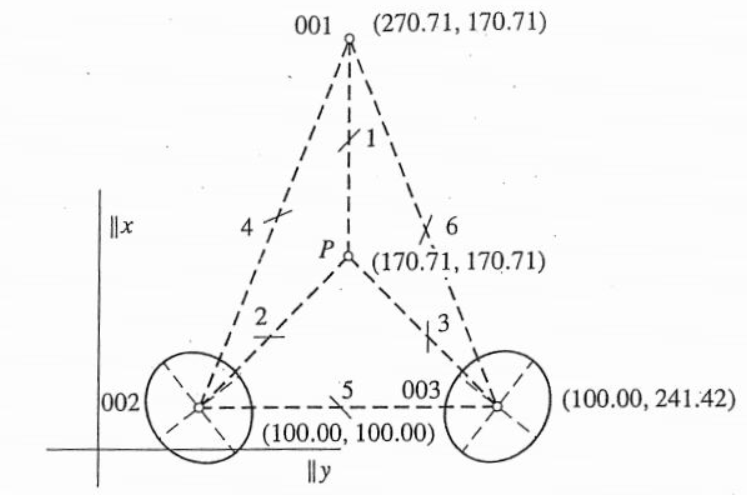
\includegraphics[width=0.4\linewidth]{TeX_files/Part02/chapter07/image/7-3.png}
	\caption{}
	\label{fig:7-3}
\end{figure}
\par\noindent
\textbf{Figure 7.3} Free distance network with 6 observations. The confidence ellipses correspond to the postulated coordinates $X_P$,$Y_P$,$X_{001}$,and $Y_{001}$.
\par\noindent
more observations compared to Example 7.1. For reasons of symmetry we include even three more observations, viz. distance observations between the pairs 001-002, 002-003,and 003-001. The vector of unknowns is
\begin{equation*}
	x =
	\begin{pmatrix}
		x_P,y_P,x_{001},y_{001},x_{002},
		y_{002},x_{003},y_{003}
	\end{pmatrix}.
\end{equation*}
The augmented coefficient matrix is 6 by 8 with rank 4:
\begin{equation*}
	A =
	\begin{bmatrix}
		-1 & 0 & 1 & 0 & 0 & 0 & 0 & 0\\
		0.707 & 0.707 & 0 & 0 & -0.707 & -0.707 & 0 & 0\\
		0.707 &-0.707& 0 &0 &0& 0& -0.707& 0.707\\
		0 & 0 &0.924& 0.383& -0.924 &-0.383& 0& 0\\
		0& 0 &0 &0 &0 &-1& 0& 1\\
		0& 0 &0.924 &-0.383& 0& 0&\ -0.924& 0.383
	\end{bmatrix}.
\end{equation*}
We choose a basis for the nullspace of dimension 4, in the rows of $G^\mathsf{T}$:
\begin{equation*}
	G^\mathsf{T} =
	\begin{bmatrix}
		1 & 0 & 1 & 0 & 1 & 0 & 1 & 0\\
		0 & 1 & 0 & 1 & 0 & 1 & 0 & 1\\
		-170.71 & 170.71 &-170.71& 270.71& -100 &100& -241.42& 100\\
		\quad170.71& 170.71 &\quad270.71 &170.71& \quad100& 100& 100& \quad241.42
	\end{bmatrix}.
\end{equation*}
and the right side is
\begin{equation*}
	b
	=\begin{bmatrix}
		0.010\\
		0.020\\
		0.030\\
		0.010\\
		0.020\\
		0.030
	\end{bmatrix}.
\end{equation*}
The pseudoinverse solution $x^+ = A^+b$ and the residuals $b - Ax^+$ are
\begin{equation*}
	b
	=\begin{bmatrix}
		\quad 0.008 0\\
		\quad0.002 3\\
		\quad0.0113\\
		-0.0068\\
		-0.0026\\
		-0.0087\\
		-0.0167\\
		0.013 2
	\end{bmatrix}
	\qquad \text{and}  \qquad
	b- Ax^+
	=\begin{bmatrix}
		\quad0.0067\\
		\quad0.0047\\
		\quad0.0047\\
		-0.0036\\
		-0.0020\\
		-0.0036
	\end{bmatrix}.
\end{equation*}
The standard deviation is $\hat{\sigma_0} = 10.9mm$. The least-squares solution of the free network yields the following coordinates$(X_{i}^{'},Y_{i}^{'})$:
\par
\begin{tabular}{ccccccc}
	Point & $X_i$ & $\xi_i$ & $X_{i}^{'}$ & $Y_i$ & $\eta_i$ & $Y_{i}^{'}$\\
	\hline
	P & 170.71 & 0.008 & 170.718 & 170.71 &\quad 0.002 &170.71\\
	1 &270.71  & 0.011 &270.721  &170.71  &-0.007 &170.703\\
	2 &100.00  &-0.003 &99.997   &100.00  &-0.009 &99.991\\
	3 &100.00  &-0.017 &99.983   &241.42  &\quad0.013  &241.433
\end{tabular}
\par\noindent

Note that $\sum{\xi_{i}} = \sum_{\eta_i} = 0$ within the computational accuracy.	= 
\begin{equation*}
\begin{bmatrix}
		\quad0.0067\\
		\quad0.0047\\
		\quad0.0047\\
		-0.0036\\
		-0.0020\\
		-0.0036
	\end{bmatrix}.
\end{equation*}
The standard deviation is $\hat{\sigma_0} = 10.9mm$. The least-squares solution of the free network yields the following coordinates$(X_{i}^{'},Y_{i}^{'})$:
\par
\begin{tabular}{ccccccc}
	Point & $X_i$ & $\xi_i$ & $X_{i}^{'}$ & $Y_i$ & $\eta_i$ & $Y_{i}^{'}$\\
	\hline
	P & 170.71 & 0.008 & 170.718 & 170.71 &\quad 0.002 &170.71\\
	1 &270.71  & 0.011 &270.721  &170.71  &-0.007 &170.703\\
	2 &100.00  &-0.003 &99.997   &100.00  &-0.009 &99.991\\
	3 &100.00  &-0.017 &99.983   &241.42  &\quad0.013  &241.433
\end{tabular}
\par\noindent
Note that $\sum{\xi_{i}} = \sum_{\eta_i} = 0$ within the computational accuracy.